\documentclass[12pt]{article}

% 基本包
\usepackage{xeCJK}
\usepackage{graphicx}
\usepackage{amsmath}
\usepackage{amssymb}
\usepackage{hyperref}
\usepackage{geometry}
\usepackage{setspace}
\usepackage{enumitem}
\usepackage{booktabs}
\usepackage{multirow}
\usepackage{float}
\usepackage{subcaption}
\usepackage{listings}
\usepackage{xcolor}
\usepackage{algorithm}
\usepackage{algorithmic}
\usepackage[backend=bibtex,style=numeric]{biblatex}
\addbibresource{references.bib}

% 設置中文字體
\setCJKmainfont{Heiti TC}
\setCJKsansfont{Heiti TC}
\setCJKmonofont{Heiti TC}

% 統一設定列表間距
\setlist{noitemsep,topsep=4pt}

% 頁面設置
\geometry{a4paper, margin=1in}
\onehalfspacing
\setlength{\parindent}{2em}  % 設定段落第一行縮排為兩個中文字寬度

% 超連結設置
\hypersetup{
    colorlinks=true,
    linkcolor=black,
    filecolor=magenta,      
    urlcolor=cyan,
    pdftitle={pdf title},
    pdfauthor={Raiso Liu},
    pdfsubject={pdf subject},
    pdfkeywords={pdf keywords}
}

% 代碼塊設置
\lstset{
    frame=none,
    breaklines=true,
    postbreak=\raisebox{0ex}[0ex][0ex]{\ensuremath{\hookrightarrow\space}},
    basicstyle=\ttfamily\scriptsize,
    keywordstyle=\color{blue},
    stringstyle=\color{red},
    commentstyle=\color{green!60!black},
    showstringspaces=false,
    backgroundcolor=\color{gray!5},
    xleftmargin=0em,
    xrightmargin=0em,
    linewidth=0.95\textwidth,
    captionpos=b
}

% 設定所有 listings 環境
\renewcommand{\lstlistingname}{Code}
\renewcommand{\lstlistlistingname}{Code List}

% 文檔信息
\title{MaskGIT Report}
\author{劉宇舜\\Department of Computer Science and Information Engineering\\National Yang Ming Chiao Tung University}
\date{\today}

\begin{document}

% 添加封面
\begin{titlepage}
    \begin{center}
        \vspace*{2cm}
        
        \Huge
        \textbf{Value-based Reinforcement Learning}
        
        \vspace{1.5cm}
        
        \Large
        \textbf{劉宇舜 Yu-Shun Liu}
        
        \vspace{1cm}
        
        \large
        Student ID: 413551030
        
        \vspace{2cm}
        
        \large
        Department of Computer Science and Information Engineering\\
        National Yang Ming Chiao Tung University
        
        \vspace{1cm}
        
        \large
        Course: Deep Learning
        
        \vspace{1cm}
        
        \large
        \today
        
    \end{center}
\end{titlepage} 

% 添加目錄
\setcounter{tocdepth}{2}
\tableofcontents
\newpage

% 添加報告內容
\section{Introduction}
This is the introduction section. MaskGIT \cite{chang2022maskgit} is a novel approach to image generation using transformers. The transformer architecture \cite{vaswani2017attention} has revolutionized many areas of deep learning. Recent advances in vision-language models \cite{radford2021learning} have shown promising results in various tasks.


\section{Implementation Details}
This is the implementation details of the project.

\subsection{Dataset}
This is the dataset used in the project.

\subsection{Model}
This is the model used in the project.


\clearpage
\section{Analysis and Discussion}


\subsection{Task1}
首先我在這次的作業中理解到 batch size 不是越大越好。
不論是平衡車的任務還是乒乓球的任務,當我的 batch size 開到 1024 的時候,模型都學不動了。

\begin{figure}[htbp]
    \centering
    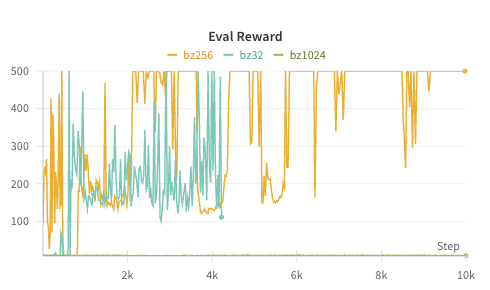
\includegraphics[width=0.8\textwidth]{figures/Eval_Reward.png}
    \caption{不同 batch size 下的評估獎勵曲線。}
    \label{fig:eval_reward}
\end{figure}

從圖 \ref{fig:eval_reward} 中可以看到,當 batch size 為 1024 時,模型的學習效果明顯幾乎為 0 。這可能是因為過大的 batch size 導致梯度更新過於平滑,使得模型難以跳出局部最優解。相比之下,較小的 batch size(如 256 或 512)能夠提供更好的探索能力,使模型能夠更快地找到更好的策略。


\begin{figure}[htbp]
    \centering
    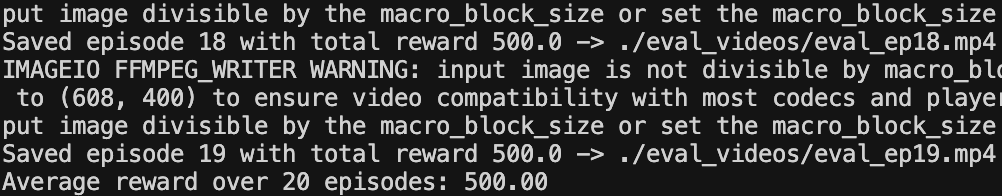
\includegraphics[width=0.8\textwidth]{figures/task1_reward.png}
    \caption{Task1 中的 Average Reward}
    \label{fig:task1_reward}
\end{figure}


最後我使用 256 的 batch size、100k 的 memory size 與 5e-5 的 learning rate 來進行訓練,在 1560 個 episodes 的時候達到了 20 次都連續 500 分的上限,如圖 \ref{fig:task1_reward}。

\subsection{Task2}

這裡我們要使用 vanilla DQN 來訓練 Pong 的遊戲,作業要我們使用視覺輸入當作網路的輸入,模擬人類真正在玩遊戲的過程,所以這裡我們需要使用 CNN 來處理視覺輸入。

模型的架構如下:
\begin{lstlisting}[language=Python, caption=用於處理視覺輸入的 CNN 模型架構。]
self.network = nn.Sequential(
    nn.Conv2d(4, 32, kernel_size=8, stride=4),
    nn.ReLU(),
    nn.Conv2d(32, 64, kernel_size=4, stride=2),
    nn.ReLU(),
    nn.Conv2d(64, 64, kernel_size=3, stride=1),
    nn.ReLU(),
    nn.Flatten(),
    nn.Linear(64 * 7 * 7, 512),
    nn.ReLU(),
    nn.Linear(512, num_actions)
)
\end{lstlisting}
這個模型接收 4 個連續的灰度圖像作為輸入(模擬時間序列),通過三個卷積層提取特徵,然後將特徵展平並通過兩個全連接層輸出每個動作的 Q 值(或分佈),然後輸出是每個 action 的預期 Reward。

由於我在訓練的時候,在每 10k env steps 的時候會執行 5 次的 evaluation。

\begin{figure}[htbp]
    \centering
    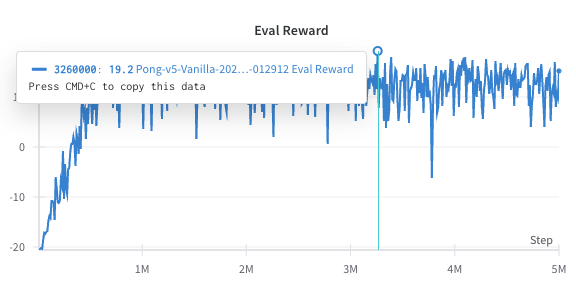
\includegraphics[width=0.8\textwidth]{figures/task2_max.png}
    \caption{Task2 中評估獎勵的最大值。}
    \label{fig:task2_max_reward}
\end{figure}

大約在 3.26 M env steps 的時候,評估獎勵達到了 19.2 分,如圖 \ref{fig:task2_max_reward}。


但是當我嘗試使用 20 次去 evaluate 的時候,發現模型會有幾次特別低分,這是其中一次執行的結果。

\begin{lstlisting}[language=Python, caption=Task2 中 20 次評估的結果,high evaluation results。]
Average reward over 20 episodes: 14.55 +/- 9.18
Individual rewards: [17.0, -21.0, 19.0, 17.0, 19.0, 17.0, 18.0, 19.0, 18.0, 7.0, 17.0, 14.0, 17.0, 21.0, 21.0, 3.0, 16.0, 18.0, 19.0, 15.0]
\end{lstlisting}

如果細看影片,就會發現,兩邊會來回對打越來越快,但是我方的 agent 並沒有利用自己橫向位移的速度優勢,而是直球對決,再加上我方的 agent 有切球的習慣,所以一個不小行,就會讓球漏過去。

所以我在檢索其他次高的 evaluation checkpoint時,找到在 3.91 M env steps 的時候,平均 20 次可以達到 16.7 分。


\begin{lstlisting}[language=Python, caption=Task2 中 20 次評估的結果,second high evaluation results。]
Average reward over 20 episodes: 16.70 +/- 3.32
Individual rewards: [15.0, 16.0, 20.0, 19.0, 8.0, 17.0, 20.0, 18.0, 16.0, 15.0, 19.0, 19.0, 10.0, 13.0, 20.0, 17.0, 19.0, 19.0, 14.0, 20.0]
\end{lstlisting}

這個結果就比較穩定,不會有特別低的分數。

\subsection{Task3}
接下來我們就採用 Rainbow DQN 的方式來訓練模型,因為這是當前最有效率探索策略的方法。


\begin{figure}[htbp]
    \centering
    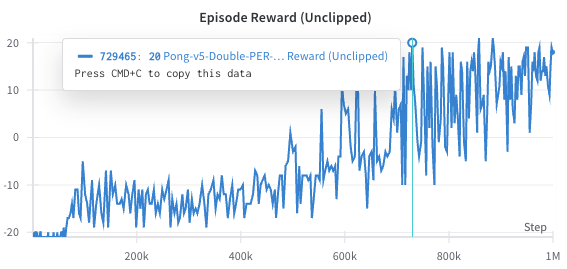
\includegraphics[width=0.8\textwidth]{figures/Task3_efficiency.png}
    \caption{Task3 中最快 over 19 分的時刻。}
    \label{fig:task3_efficiency}
\end{figure}

從圖 \ref{fig:task3_efficiency} 可以看出,Rainbow DQN 在我實作的版本中,大約需要 730k env steps 就可以達到 19 分。


\subsection{Ablation Study}

原本的要求是使用 Double DQN 、 PER 以及 Multi-step Learning 來做優化,在 Rainbow DQN 中,多了 Distributional RL 以及 Noisy Networks。

所以我嘗試把這兩個技術拿掉,看看效果如何。

\begin{figure}[htbp]
    \centering
    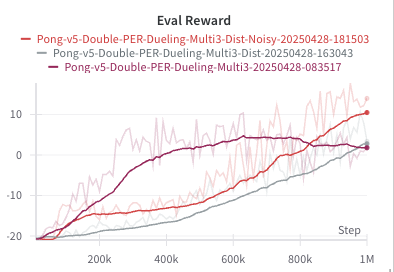
\includegraphics[width=0.8\textwidth]{figures/task3_ablation.png}
    \caption{Task3 中不同技術組合的比較。(smooth lines)}
    \label{fig:task3_ablation}
\end{figure}

從圖 \ref{fig:task3_ablation} 可以看出,首先是紫色線,是兩個技術都沒有使用,可以很快的收斂,但是我猜是次優解,所以還會越訓練越差,當我們加入 Distributional RL 之後,雖然慢,但模型可以穩定的提升,其中的振幅是這三條線中最小的,但很可惜他到了 15 分左右就上不去了,最後當我們加入 Noisy Networks 之後,模型可以穩定提升且灰色線快,這也是完整版本的 Rainbow DQN 的結果。

Note: 令我疑惑的是,在原始論文的實作中,可以在 400 k env steps 就達到 19 分,但是在我實作的版本中,卻需要 730 k env steps 才能達到 19 分,這是為什麼呢?




% 添加參考文獻
\clearpage
\printbibliography

\end{document} 